\begin{description}
\item[7.~定理.] \emph{三角形の辺を小さくしてゆくことにより、あるいは、他の二辺がある一定の長さより小さいままで一辺だけを小さくすることによってさえ、その面積を限りなく小さくでき、その角の和は二直角に限りなく近づく。}

\begin{figure}[h]
\centering
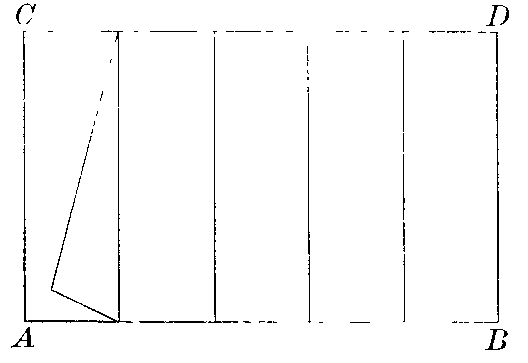
\includegraphics[width=50mm]{fig17.png}
\end{figure}

\textbf{証明.} $ABDC$ を、$A$、$B$、$C$ に三つの直角をもつ四角形とする。$AB$ に沿って動く垂線は、つねに増加するか、つねに減少する。なぜなら、もしある範囲では増加し、ある範囲では減少するとすれば、垂線が同じ長さとなる位置が異なる二つあることになり、その中間にある垂線は $CD$ にも垂直になって、長方形ができてしまうからである。

$AB$ を $n$ 個の等しい部分に分け、分点を通って垂線を引く。四角形は $n$ 個のより小さい四角形に分けられ、これらは一辺とその両端の二つの直角がすべて同じであるから、互いに重ね合わせることができる。垂線が最も短いほうの端から始めると、各四角形は、次の四角形の内部に完全に収まるように置くことができる。したがって、最初の四角形の面積は、もとの四角形の面積の $\frac{1}{n}$ より小さく、その不足あるいは過剰も、全体の不足あるいは過剰の $\frac{1}{n}$ より小さい。さて、すべての辺が $AC$ または $BD$ より小さく、かつ一辺が $AB$ の小区間の一つより小さいような任意の三角形は、この最小の四角形の内部に完全に収めることができる。そのような三角形は、その面積と、不足あるいは過剰とが、もとの四角形の面積と、不足あるいは過剰との $\frac{1}{n}$ より小さい。

こうして、三角形は、少なくとも一辺を十分に小さくとれば、他の二辺が限りなく大きくなければ、その面積と不足あるいは過剰を、どれほど小さく指定された面積と不足あるいは過剰よりも小さくできる。

\item[8.~定理.] \emph{不足あるいは過剰が同じ二つの三角形は、面積が等しい。}

\begin{figure}[h]
\centering
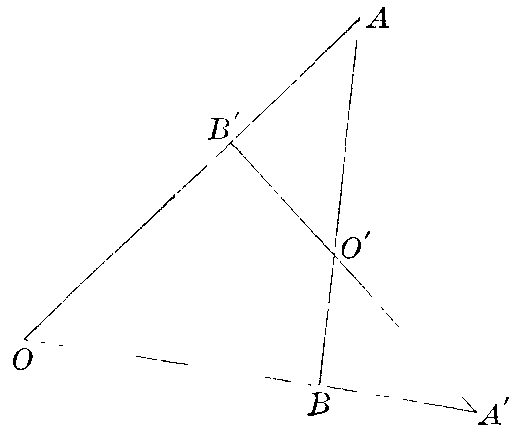
\includegraphics[width=40mm]{fig18.png}
\end{figure}

\textbf{証明.} $AOB$ と $A'OB'$ が、不足あるいは過剰が同じで、一方の一つの角が他方の一つの角に等しいとする。等しい角が重なるように二つを並べて置くと、二つの三角形は完全に重なって等しくなるか、あるいは二つに共通な四角形ができ、そのほかに、両方に共通な一つの角をもち、不足あるいは過剰が同じである二つのより小さな三角形が残る。これらを並べて置くと、ふたたび両方に共通な四角形と、両方に共通な一つの角をもち、不足あるいは過剰が同じである第三の三角形の組が得られる。この過程は、重なり合う三角形の組に出会わないかぎり、限りなく続けることができる。なぜなら、二つの三角形の不足あるいは過剰が同じであるから、組の一方の三角形が他方に完全に含まれることは、どの段階でもないからである。

最初の二つの三角形の、等しい角に対する辺の和を $so$、隣り合う辺の和を $sa$ とし、二つの三角形を並べて置いたときに両者に共通する、二度数えられる隣り合う辺の部分を $s'a$ とする。第二の三角形の組に $o'$ と $a'$、第三の組に $o''$ と $a'$、などを用いると、
\begin{gather*}
\begin{aligned}
sa   &= s'a + so',                 & so   &= sa',  \\
sa'  &= s'a' + so'',               & so'  &= sa'', \\
sa'' &= s'a'' + so'''\text{, etc.} & so'' &= sa''' \text{, etc.}
\end{aligned}\\
\begin{aligned}
\therefore sa  &= s'a  + s'a''  + s'a^{IV} + \ldots, \\
           sa' &= s'a' + s'a''' + s'a^{V}  + \ldots.
\end{aligned}
\end{gather*}

したがって、$s'a$、$s'a'$、$s'a''$、$\cdots$ は限りなく小さくなる。これらの各々は、三角形の組の一方から二度数えた一辺と、他方から二度数えた一辺とからなる。したがって、過程を十分遠くまで進めれば、残る三角形は、少なくとも一辺を望むだけ小さくでき、しかもすべての辺は小さくなって、たとえばもとの三角形の最長の辺より小さくなる。ゆえに、残る三角形の面積は限りなく小さくなるが、各組の三角形の面積の差は同じままなのだから、この差は零でなければならない。各組の三角形、とくに最初の二つの三角形は、面積が等しい。

\begin{figure}[ht]
\centering
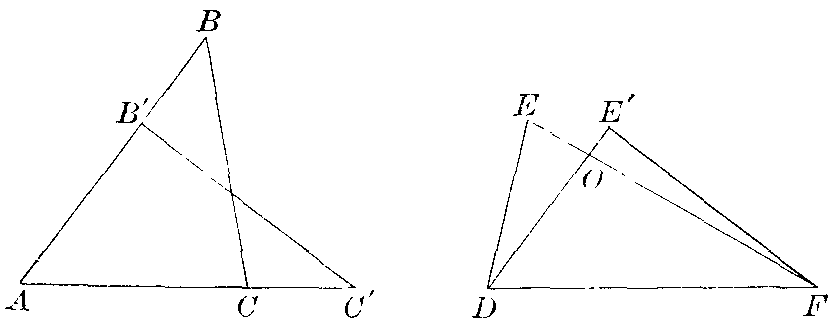
\includegraphics[width=70mm]{fig19.png}
\end{figure}

$ABC$ と $DEF$ の不足あるいは過剰が同じで、$AC<DF$ とする。$AC$ を $C'$ まで延長して $AC'$ = $DF$ とする。すると $AB$ 上の $A$ と $B$ の間に、$AB'C'$ が $ABC$ と同じ不足あるいは過剰と同じ面積をもつような点 $B'$ がある。$AB'C'$ を、$AC'$ が $DF$ に重なるように $DEF$ の上に置き、それが占める位置を $DE'F$ とする。二つの三角形が重ならなければ、共通の辺 $DF$ に対する各々の頂点は他方の外側にある。二つの三角形は共通に、たとえば三角形 $DOF$ をもち、そのほかに、二つの三角形のうちから、両方に同じ一つの角をもち、不足あるいは過剰が同じである二つのより小さな三角形が残る。この二つの三角形は、したがってもとの三角形も、面積が等しい。

\item[9.~定理.] \emph{任意の二つの三角形の面積は、それらの不足あるいは過剰に比例する。}

\begin{figure}[h]
\centering
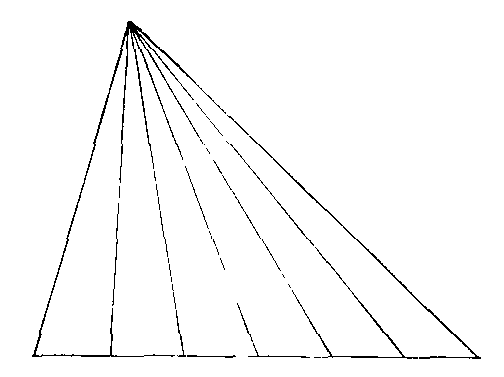
\includegraphics[width=40mm]{fig20.png}
\end{figure}

\textbf{証明.} 三角形は、一つの頂点から対辺上の点へ引いた線によって、不足あるいは過剰が等しく面積も等しい $n$ 個のより小さい三角形に分けることができる。これらの三角形の各々は、不足あるいは過剰がもとの三角形の不足あるいは過剰の $\frac{1}{n}$ であり、面積がもとの三角形の面積の $\frac{1}{n}$ である。

二つの三角形の不足あるいは過剰が通約できる、たとえば比が $m: n$ であるときは、それらを、それぞれ $m$ 個と $n$ 個の、すべて同じ不足あるいは過剰と同じ面積をもつより小さい三角形に分けることができる。与えられた三角形の面積は、したがって同じ比 $m : n$ をなす。

\begin{figure}[h]
\centering
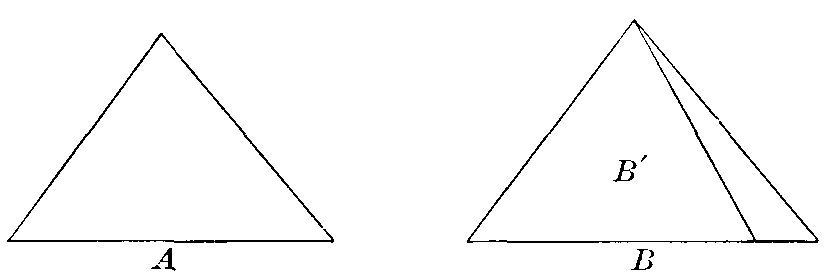
\includegraphics[width=70mm]{fig21.png}
\end{figure}

二つの三角形 $A$ と $B$ の不足あるいは過剰が通約できないときは、一方の三角形 $A$ を上のように任意の個数の等価な部分に分け、これらのうちの一つに等価な部分を、他方から、できるかぎり多くとる。すると、これらの部分の一つの不足あるいは過剰より小さい不足あるいは過剰をもつ残りができる。第二の三角形からとった部分は三角形 $B'$ をなす。$A$ と $B'$ は、不足あるいは過剰が通約できるから、面積がそれらに比例する。そこで $A$ を分ける部分の個数を限りなく増す。これらの部分は限りなく小さくなり、$B$ から $B'$ をとった残りも限りなく小さくなる。$B'$ の不足あるいは過剰と面積は、$B$ のそれらに近づき、三角形 $A$ と $B$ の面積は、それらの不足あるいは過剰に比例する。

\textbf{系.} \emph{二つの多角形の面積の比は、それらの不足あるいは過剰の比に等しい。}

\item[10.~定理.] \emph{一つの角を固定した直角三角形において、三角形の辺を限りなく小さくしてゆくとき、斜辺に対する対辺の比と斜辺に対する隣辺の比は、その角の正弦と余弦に極限として近づく。}

\textbf{証明.} 斜辺上に、任意個の等しい長さをとる。分点 $A_1$、$A_2$、$\cdots$ を通って底辺に垂線 $A_1C_1$、$A_2C_2$、$\cdots$ を引き、これらの線の延長に対して、斜辺の次の分点からそれぞれ垂線 $A_2D_1$、$A_3D_2$、$\cdots$ を引く。

三角形 $OA_1C_1$ と $A_2A_1D_1$ は等しい（II, 6, 系）。
\begin{align*}
  C_2A_2 &\gtrless C_1D_1 &&\text{かつ} & C_1C_2 &\lessgtr D_1A_2;\\
  \intertext{したがって、}
  \frac{C_2A_2}{OA_2} &\gtrless \frac{C_1A_1}{OA_1}
  &&\text{かつ} & \frac{OC_2}{OA_2} &\lessgtr \frac{OC_1}{OA_1},
\end{align*}
上側の符号は第二の仮説、下側の符号は第三の仮説に対応する。

\begin{figure}[h]
\centering
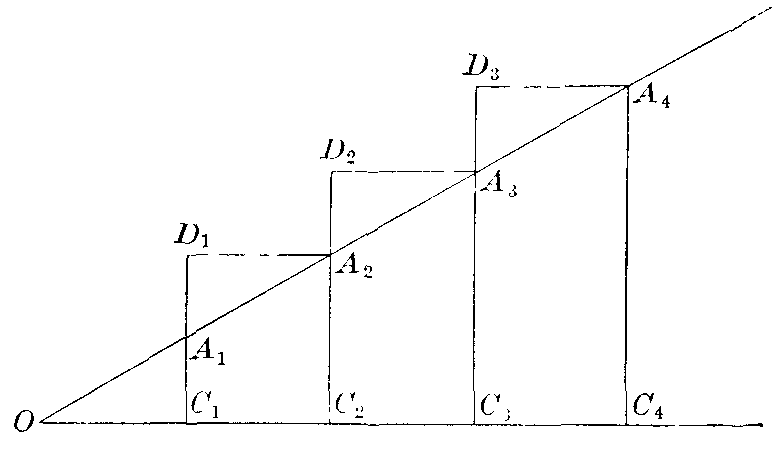
\includegraphics[width=70mm]{fig22.png}
\end{figure}

つぎを仮定する。
\begin{equation*}
  \frac{C_{r-1}A_{r-1}}{OA_{r-1}}
  \gtrless \frac{C_{r-2}A_{r-2}}{OA_{r-2}}
  \gtrless \dots
  \gtrless \frac{C_1A_1}{OA_1},
\end{equation*}
および
\begin{equation*}
  \frac{OC_{r-1}}{OA_{r-1}}
  \lessgtr \frac{OC_{r-2}}{OA_{r-2}}
  \lessgtr \dots
  \lessgtr \frac{OC_1}{OA_1}.
\end{equation*}

\begin{align*}
  OA_{r-1} &= (r-1) OA_1,\\
\intertext{かつまた}
           &= (r-1) A_{r-1}A_r,
\end{align*}
であるから、不等式
\begin{equation*}
  \frac{OC_1}{OA_1} \gtrless \frac{OC_{r-1}}{OA_{r-1}} \quad
  \text{および}\quad
  \frac{C_1A_1}{OA_1} \lessgtr \frac{C_{r-1}A_{r-1}}{OA_{r-1}}
\end{equation*}
を $A_{r-1}$ での角に適用すると、
\begin{equation*}
  \frac{A_{r-1}D_{r-1}}{A_{r-1}A_r} \gtrless
  \frac{C_{r-1}A_{r-1}}{OA_{r-1}}\quad
  \text{および}\quad
  \frac{D_{r-1}A_r}{A_{r-1}A_r} \lessgtr
  \frac{OC_{r-1}}{OA_{r-1}}
\end{equation*}
となる。

この二つの不等式のうち第一のものは、つぎのように書ける。
\begin{equation*}
  \frac{A_{r-1}D_{r-1}}{C_{r-1}A_{r-1}} \gtrless
  \frac{A_{r-1}A_r}{OA_{r-1}}.
\end{equation*}

両辺に 1 を加えると、
\begin{align*}
\frac{C_{r-1}D_{r-1}}{C_{r-1}A_{r-1}} &\gtrless
                                            \frac{OA_r}{OA_{r-1}}, \\
\intertext{すなわち}
\frac{C_{r-1}D_{r-1}}{OA_r} &\gtrless
                                   \frac{C_{r-1}A_{r-1}}{OA_{r-1}}, \\
\intertext{しかるに}
C_rA_r &\gtrless C_{r-1}D_{r-1}, \\
\intertext{したがって}
\frac{C_rA_r}{OA_r} &\gtrless \frac{C_{r-1}A_{r-1}}{OA_{r-1}}, \\
\end{align*}

またさらに、
\begin{align*}
C_{r-1}C_r &\lessgtr D_{r-1}A_r. \\
\intertext{ゆえに、上の第二の不等式から、}
\frac{C_{r-1}C_r}{A_{r-1}A_r} &\lessgtr \frac{OC_{r-1}}{OA_{r-1}}, \\
\intertext{すなわち}
\frac{C_{r-1}C_r}{OC_{r-1}} &\lessgtr \frac{A_{r-1}A_r}{OA_{r-1}}. \\
\end{align*}

両辺に 1 を加えると、
\begin{align*}
\frac{OC_r}{OC_{r-1}} &\lessgtr \frac{OA_r}{OA_{r-1}}, \\
\intertext{すなわち}
\frac{OC_r}{OA_r} &\lessgtr \frac{OC_{r-1}}{OA_{r-1}}
\end{align*}
となる。

比 $\dfrac{CA}{OA}$ と $\dfrac{OC}{OA}$ は 1 より小さく、斜辺が減少するとき、つねに増加するかつねに減少するから、確定した極限に近づく。これらの極限は $A$ の連続関数である。実際、任意の直角三角形の角を連続的に変化させ、斜辺をある一定の長さに保つと、他の二辺は連続的に変化するから、斜辺に対するそれらの比の極限も、連続的に変化しなければならない。

これらの極限をさしあたり $sA$ と $cA$ と呼ぶことにして、三角法でのように、その定義を任意の角に拡張し、正弦と余弦の公式がすべてこれらの関数についても成り立つことを証明できる。そして、特定の角 $30^\circ$、$45^\circ$、$60^\circ$ について、それらが正弦と余弦と同じ値をもつことを証明でき、他のすべての角でのそれらの値は、これらの角での値から定まるから、正弦と余弦の対応する値と同じになる。

\begin{figure}[ht]
\centering
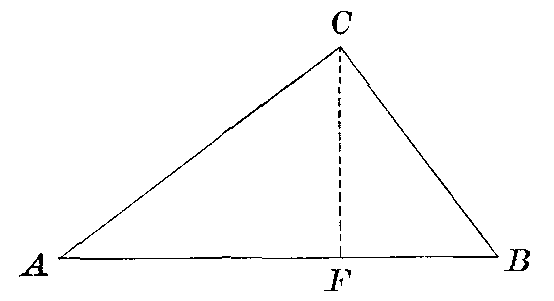
\includegraphics[width=50mm]{fig23.png}
\end{figure}

直角 $C$ から斜辺 $AB$ へ垂線 $CF$ を引く。角 $FCB$ は $A$ に等しくないが、その差は、二つの三角形 $ABC$ と $FBC$ の面積の差に比例するから、三角形の辺が小さくなるとき限りなく小さくなる。関係
\begin{equation*}
\frac{AF}{AC}\cdot\frac{AC}{AB} +
    \frac{FB}{BC}\cdot\frac{BC}{AB} = 1
\end{equation*}
から、極限へ移ると、
\begin{equation*}
(cA)^2 + (sA)^2 = 1
\end{equation*}
を得る。

$x$ と $y$ を任意の二つの鋭角とし、二つの角の和の正弦と余弦の公式を証明するのに用いる図を描く。

角 $x$ と $y$ を固定したまま、すべての線を限りなく小さくすることを考えることができ、関数 $sx$、$cx$、$sy$ などは、これらの線のある比の極限である。
\begin{gather*}
\begin{aligned}
\frac{CA}{OA} &= \frac{CE}{OB}\cdot\frac{OB}{OA}
                                + \frac{EA}{BA}\cdot\frac{BA}{OA}, \\
\pm \frac{CA}{OA} &= \frac{OD}{OB}\cdot\frac{OB}{OA}
                                - \frac{CD}{BA}\cdot\frac{BA}{OA}, \\
\end{aligned} \\
\left(\text{第二の図では} -\frac{OC}{OA} \right).
\end{gather*}

二つの三角形 $EMB$ と $CMO$ では $M$ での角が等しく、つぎのように書ける。
\begin{equation*}
\frac{CM}{OM} = \frac{ME + \delta}{MB}
                              = \frac{ME \pm CM + \delta}{MB \pm OM},
\end{equation*}
ここで $\delta$ の極限は零である。
\begin{equation*}
\therefore \lim \frac{CE}{OB} = \lim\frac{CM}{OM} = sx.
\end{equation*}

\begin{figure}[h]
\centering
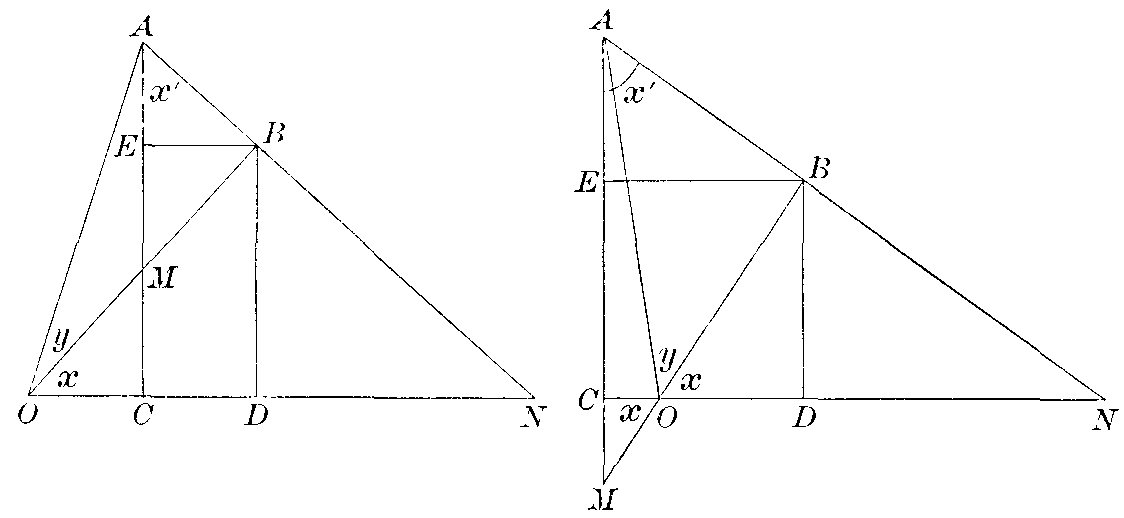
\includegraphics[width=80mm]{fig24.png}
\end{figure}

角 $EAB$、すなわち $x'$ は $x$ と同じではないが、$x$ との差は、三角形 $OMC$ と $MAB$ の面積の差に比例する量にすぎず、したがって限りなく小さくなる。こうして $sx'$ と $cx'$ の極限は $sx$ と $cx$ である。

最後に、二つの三角形 $ACN$ と $BDN$ が角 $N$ を共有するから、つぎのように書ける。
\begin{equation*}
\frac{DN}{BN} = \frac{CN + \delta '}{AN}
                                = \frac{CN - DN + \delta '}{AN - BN},
\end{equation*}
ここで $\delta'$ の極限は零である。
\begin{equation*}
\therefore \lim \frac{CD}{AB} = \lim\frac{CN}{AN} = sx.
\end{equation*}

さて極限において、恒等式は
\begin{align*}
s(x+y) &=  sx \cdot cy + cx \cdot sy, \\
c(x+y) &=  cx \cdot cy - sx \cdot sy
\end{align*}
となる。

帰納法によって、これらの公式は任意の角について真であることが証明される。これらの関数の値を $30^\circ$、$45^\circ$、$60^\circ$ での値から計算するのに十分な他の公式は、この二つから代数的な操作で得られる。

直角二等辺三角形の辺が限りなく小さくなるとき、角は固定されたままではなく $45^\circ$ に近づき、斜辺に対する二辺の比は、極限 $s\ 45^\circ$ と $c\ 45^\circ$ に近づく。したがって、これらは等しく、それらの平方の和は 1 であるから、それぞれの値は $\frac{1}{\sqrt{2}}$ であり、$45^\circ$ の正弦と余弦の値と同じである。

また、正三角形を二等分して、斜辺が一辺の二倍となる三角形をつくる。この関係を保ったまま辺を小さくしてゆくと、角は $30^\circ$ と $60^\circ$ に近づく。したがって、これらの角の関数 $s$ と $c$ の値は、同じ角の正弦と余弦の対応する値と同じである。

\textbf{系.} \emph{平面三角形が限りなく小さくなるとき、辺と角の関係は、われわれになじみのある通常の幾何学と三角法の平面三角形の辺と角の関係に近づく。}

\item[11.~定理.] \emph{球面幾何学は三つの仮説において同じであり、球面三角法の公式は通常の球面三角法のものとまったく同じである。}

\textbf{証明.} 球面上では、大円の弧は、それが中心に対する角に比例し、球面上の角は、その角の辺である大円の平面がなす二面角に等しい。それらの関係は、望むだけ小さくできる、したがって直角の仮説における平面三角形のようであると仮定してよい、ある平面三角形を描くことによって確立される。ゆえに、これらの関係は通常の球面三角法のものである。
\end{description}

\medskip 三つの仮説は、三つの幾何学の体系を生じ、それらは放物幾何学、双曲幾何学、楕円幾何学と呼ばれる。これらはまた、ユークリッドの幾何学、ロバチェフスキーの幾何学、リーマンの幾何学とも呼ばれる。次のような考察は、それらの主な特徴のいくつかを示す。

\begin{figure}[h]
\centering
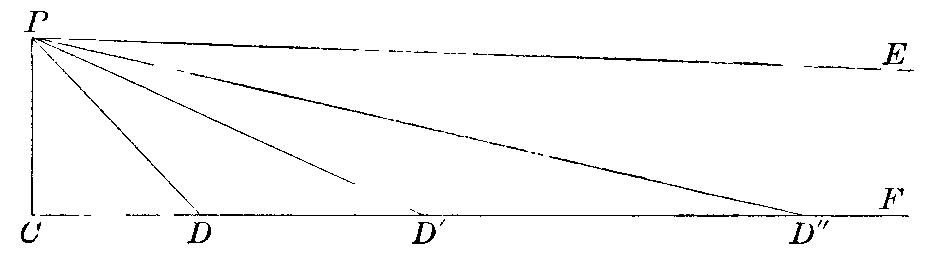
\includegraphics[width=80mm]{fig25.png}
\end{figure}

直線 $CF$ に垂直な $PC$ が与えられたとする。この直線上に、
\begin{align*}
  CD    &= PC, \\
  DD'   &= PD, \\
  D'D'' &= PD',\ \text{など}
\end{align*}
をとる。

さて $PC$ が十分に短い（限定されている）ならば、それは $P$ から直線 $CF$ に至る\emph{他のどんな}線よりも短い。なぜなら、$PC$ 以下の短さの線はどれも、点 $P$ のまわりの平面の限定された部分に含まれ、その部分では、垂線が点から直線への最短距離だからである。

したがって、
\begin{align*}
  PD  &> PC,               &\therefore CD' &> 2CD,\\
  PD' &> PC,\ \text{など;} &          CD'' &> 3CD,\ \text{など}
\end{align*}

またさらに、三つの仮説において、それぞれ、
\begin{align*}
  CPD    &\stackrel{=}{\lessgtr} \frac{\pi}{4}, &&\text{かつ}&
                         CDP &\stackrel{=}{\lessgtr} \frac{\pi}{4},\\
  DPD'   &\stackrel{=}{\lessgtr} \tfrac{1}{2} CPD, &&&
                    CD'P  &\stackrel{=}{\lessgtr} \tfrac{1}{2} CDP,\\
  D'PD'' &\stackrel{=}{\lessgtr} \tfrac{1}{2} DPD',\ \text{など,} &&&
        CD''P &\stackrel{=}{\lessgtr} \tfrac{1}{2} CD'P,\ \text{など}
\end{align*}

$P$ には一連の角ができる。第一の仮説では、これらの角は無限に多くあり、その列は公比 $\frac{1}{2}$ の等比数列をなし、その和はちょうど $\frac{\pi}{2}$ である。第二の仮説でも、これらの角は無限に多くあり、列の各項は等比数列の各項より小さい。したがって、その列の和は $\frac{\pi}{2}$ より小さい。第三の仮説では、各項が等比数列の各項より大きい列ができ、したがって、その列が収束するか発散するかにかかわらず、十分な数の項をとれば $\frac{\pi}{2}$ より大きくなる。いいかえれば、この過程を有限の回数くり返すことによって、$P$ に直角か、それより大きな角が得られる。

$D$、$D'$、$D''$、$\cdots$ での角は、$P$ での角の列の各項にちょうど等しい。最初の二つの仮説では、それらは極限として零に近づく。

距離 $CD$、$CD'$、$CD''$、$\cdots$ は、毎回、ある確定した量 $CD$ より多く増加する。したがって、この過程を限りなくくり返すと、これらの距離はあらゆる限界を超えて増大する。こうして、第一および第二の仮説では、直線が無限の長さをもたなければならないことが証明される。

鈍角の仮説では、$PC$ に点 $P$ で垂直な線は、$C$ から有限のある距離にある点、すなわち $D$ のどれか、またはその間のある点で、$CF$ と交わる。$PC$ の反対側でも、この同じ垂線は、延長した $FC$ と同じ距離のところで交わる。しかし、二つの異なる直線が二点で交わることはないと仮定してあるから、われわれにとって第三の仮説は、直線が有限の長さをもち、それ自身に戻る場合にのみ真でありうる。このとき、これら二つの点は同一の点であり、その $C$ からの距離は、どちらの向きでも直線全体の長さの半分である。しかし、このようにして、第三の仮説の上に無矛盾な幾何学を築くことができ、この幾何学が楕円幾何学と呼ばれるものである。

作図は、$CF$ 上に任意の長さの $CD$ をとっても同じであり、ほとんどすべての叙述も同じになったはずである。

この章の命題のいくつかに課した制限は、第三の仮説では必要である。

\begin{figure}[h]
\centering
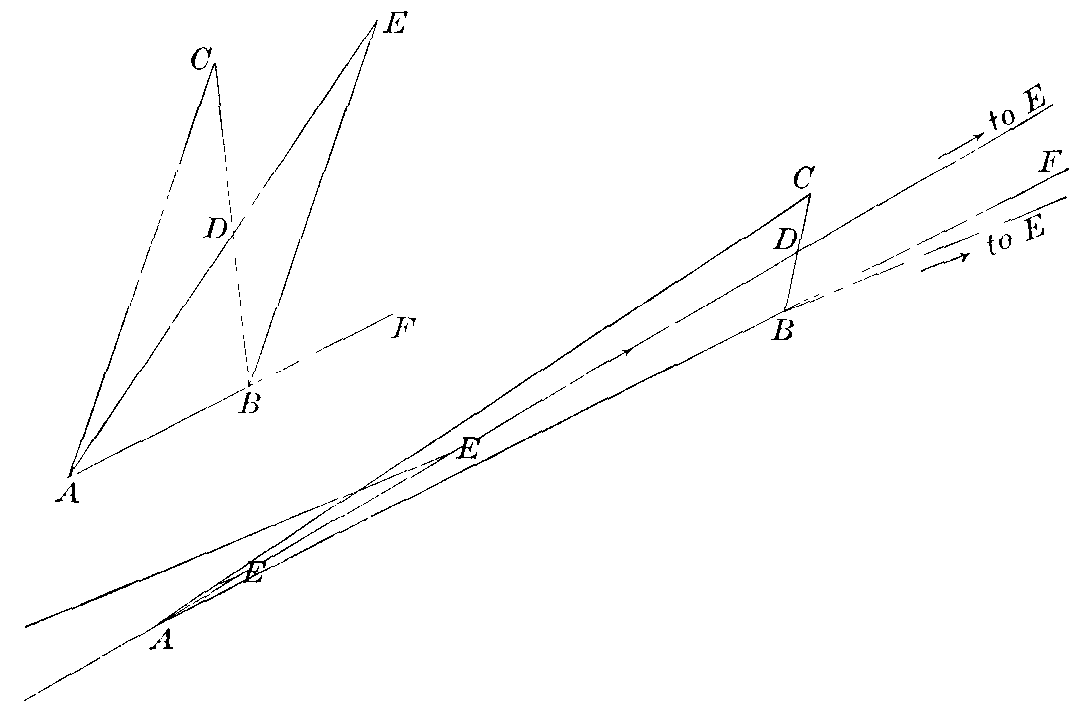
\includegraphics[width=80mm]{fig26.png}
\end{figure}

たとえば、三角形の外角が隣り合わない内角より大きいことの証明では、頂点 $A$ から対辺の中点 $D$ へ引いた線 $AD$ を、$AE=2AD$ となるように延長した。$AD$ が、$A$ と $D$ で定まる直線の全長の半分より大きければ、これは点 $E$ を点 $A$ の先へ持ってゆくことになり、角 $C$ に等しい角 $CBE$ は、外角 $CBF$ の一部となる代わりに、この外角より大きくなる。

\begin{figure}[h]
\centering
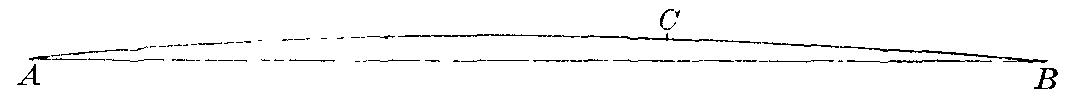
\includegraphics[width=80mm]{fig27.png}
\end{figure}

また、三角形の二つの角が等しく、その間の辺がちょうど直線全体であるときは、対辺が等しいことは必ずしも導かれない。しかし、その対辺は一つの連続した線をなすのだから、この図形は厳密には三角形ではなく、むしろ月形に似た図形であるともいえる。点 $A$ と $B$ は同じ点であり、角 $A$ と $B$ は対頂角である。

最後に、二点間の最短の道は直線であると仮定してはいるが、二点の間に引いた直線がつねにその二点間の最短の道であるとは限らない。直線上で一方の点から他方へ行く方法は二通りある。すなわち、二点がその決める直線を分けてできる二つの部分のそれぞれを通る道である。これらの部分の一方は通常は他方より短く、長いほうの部分は、折れ線や曲線に沿ったいくつかの道より長くなる。

しかし、直線が無限の長さをもつとき、すなわち直角の仮説と鋭角の仮説においては、この章の命題はすべて制限なしに成り立つ。

\medskip ユークリッド幾何学はだれにもなじみ深い。つぎにロバチェフスキーの幾何学を詳しく調べ、そのあと同じ方法で楕円幾何学を取り上げよう。
